\scanpage{81}
% archive sheet number: 80
\[
y=z\qquad x=(1+\alpha')y=-\alpha y\qquad y=\alpha'x
\]
\[
\begin{aligned}
\underline{(-\alpha y,y,y)}&\quad\text{ou}\quad(x,\alpha'x,\alpha'x)\\
(-\alpha,1,1)&\qquad(1,\alpha',\alpha')\\
-\alpha&=\alpha'(1-\alpha')=\alpha'-\alpha'^2\\
\alpha'&\overset{?}{=}-\alpha(1-\alpha')=-\alpha-1\quad\text{OK}
\end{aligned}
\]
\margin{$\begin{aligned}1-(2-\alpha)\\\alpha-1\\\alpha=\tfrac12\\\tfrac14+\tfrac12-1=0\\1+2-4=0\\-1=0\\\unsure{\infty}\end{aligned}$}
\[
e_1\ \unsure{\text{non.}}\qquad
\left\{\begin{aligned}
\bar S_0&=(-\alpha,1,1)\\
\bar S_1&=\sigma_0\bar S_0=(\alpha-1,1,1)\\
\deleted{\unsure{e}}\quad\bar S_{\unsure{1|2}}-\bar S_0&=(\underline{2\alpha-1},0,0)
\end{aligned}\right.
\]
\[
\unsure{\alpha'^2|\alpha^2}=1-\alpha'\qquad \alpha+\alpha'=-1
\]
\margin{$\begin{aligned}\deleted{2\alpha}\ 2\\2\alpha-1=2\alpha+2-3\\\deleted{\unsure{\alpha-2}}
\end{aligned}$}
\[
\unsure{\underline{O}_S|\mathcal O_S}\quad(-\alpha,1,1)
\]
\figure{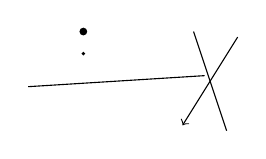
\begin{tikzpicture}[scale=.7]
\fill(1,1)circle(2pt);\fill(1,.6)circle(1pt);
\draw(0,0)--(3.2,.2);\draw(3,1)--(3.6,-.8);\draw[->](3.8,.9)--(2.8,-.7);
\end{tikzpicture}}
\[
\begin{aligned}y+z+1&=0\\x+y+\alpha z&=0\\y&\underline{=z}\end{aligned}
\qquad f(0)=f(\sigma_1\sigma_2)=0
\]
\[
\begin{aligned}f(\sigma_0^2)&=f(\sigma_0)+\sigma_0f(\sigma_0)=0\\
e+\sigma_0e&=0\\\boxed{\sigma_0e=-e}
\end{aligned}
\]
\diagram{\begin{tikzcd}[ampersand replacement=\&]
\&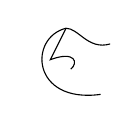
\begin{tikzpicture}[scale=.4]
\draw (1.4,0) .. controls (-.8,-.3) and (-.9,1.8) .. (.3,2.1) .. controls (.7,2.1) and (1,1.4) .. (1.7,1.6);
\draw (.3,2.1)--(-.2,1.1) .. controls (.6,1.4) and (.7,1) .. (.45,.8);
\end{tikzpicture}\\
\unsure{\Gamma|\mathscr G}\arrow[r]\&SO^{\unsure{\uparrow|+}}(q)
\end{tikzcd}}
$+\ 1$-cocycle
\[
\left\{\begin{aligned}
\Gamma&\overset{\unsure{f}}{\longrightarrow} E\\
f(gg')&=f(g)+gf(g')
\end{aligned}\right.
\]
Il suffit de donner
\[
f(\sigma_1)=f(\sigma_2)=0\qquad \unsure{C|f}(\sigma_0)=e\deleted{\unsure{q}}
\qquad\boxed{q_0(e)=1}
\]
\diagram{\begin{tikzcd}[ampersand replacement=\&,column sep=small,row sep=small]
\&S_2\&\\S_0\arrow[rr,no head]\&\&S_1
\end{tikzcd}}
\[
\begin{aligned}S_2-S_0\\=\\e_2-e_3\\(0,1,-1)\end{aligned}
\]
\[
\sigma_0\sigma_2\sigma_0\sigma_2
\]
\[
\begin{aligned}f(\sigma_0\sigma_2)&=\deleted{\unsure{e+}}e\\
f&\qquad e+\sigma_0\sigma_2e=0\\
\deleted{\boxed{\sigma_0\sigma_2e=\deleted{\unsure{\sigma_2}}-e}}\\
&=\sigma_0e\\
\sigma_0(\sigma_2e-e)&=0
\end{aligned}
\]
\[
\sigma_0\sigma_1=u\qquad
\begin{aligned}
f(u)&=e\\f(u^2)&=e+ue\\f(u^3)&=e+ue+
\end{aligned}
\]
\[
\left\{\begin{aligned}\underline{e_1\wedge e_2\wedge e_3}\\q\end{aligned}\right.
\qquad
\begin{aligned}
f(u^3)&=f(uu^2)=\\&e+u(e+ue)\\&=e+ue+u^2e=0
\end{aligned}
\]
\[
1+1+\alpha=2+\alpha=\deleted{\unsure{\alpha}}1-\alpha'=\boxed{\alpha'^2}
\]
\[
\boxed{\left\{\begin{aligned}\sigma_0e&=-e\\\sigma_2e&=e\end{aligned}\right.}
\quad\begin{aligned}\Longleftrightarrow(1+\sigma_0)e&=0\\\Longleftrightarrow(1+\sigma_0\sigma_2)e&=0\end{aligned}
\qquad\boxed{(1+u+u^2)e=0}
\]
\[
\deleted{\unsure{(1+u+u^2)e}}\qquad
\deleted{(1+u+u^2+u^3+u^4)e=0}\quad\unsure{\zeta|\}}
\]
